\textbf{1.MATLAB code for function ill (ill.m):}
\begin{lstlisting}[language=Matlab]
function y = ill(t,x)
k=1;l=0.5;
y=[k*x(1)*x(2)-l*x(1);-k*x(1)*x(2)];
end
\end{lstlisting}\nline%
%
\textbf{2.MATLAB code for solve ill (sill.m):}
\begin{lstlisting}[language=Matlab]
ts=0:50;
x0=[0.01;0.80]
[t,x]=ode45('ill',ts,x0);[t,x]
figure(1);clf;hold on;
plot(t,x(:,1),'-r','LineWidth',2);
plot(t,x(:,2),'-.b','LineWidth',2);
plot(t,1-x(:,1)-x(:,2),'--g','LineWidth',2);
xlabel('t');ylabel('i,s,r');
legend('i(t)','s(t)','r(t)');grid on;%pause
figure(2);
plot(x(:,2),x(:,1),'LineWidth',2);
xlabel('s');ylabel('i');
legend('i(s)');grid on;hold off;
\end{lstlisting}\nline%
%
\textbf{3.MATLAB code for function ill2 (ill2.m) when taken
isolution:} \begin{lstlisting}[language=Matlab]
function y = ill2(t,x)
k=1;l=0.6;
y=[k*x(1)*x(2)-l*x(1);-k*x(1)*x(2)];
end
\end{lstlisting}\nline%
%
\textbf{4.MATLAB code for study the effect of different time of
begin taking isolation for spread:}
\begin{lstlisting}[language=Matlab]
dur=50;
ts=0:dur;
x0=[0.01;0.90];
figure(1);
[t,x]=ode45('ill',ts,x0);
plot(t,x(:,1),'r-.');
xlabel('t');ylabel('i');
hold on;
figure(2);clf;
plot(x(:,2),x(:,1),'r*-.');
hold on;
for g=1:(dur/3)
    [t,xx]=ode45('ill2',ts((g+1):dur),x(g,:));
    figure(1);
    plot(t,xx(:,1));
    figure(2);
    plot(xx(:,2),xx(:,1));
end
xlabel('s');ylabel('i');
legend('no isolation','isolation');
hold off;
figure(1);
legend('no isolation','isolation');
hold off;
\end{lstlisting}\nline%
%
\textbf{5.MATLAB code for statistic data and fitting:}
\begin{lstlisting}[language=Matlab]
t=load('day_sum.txt');
s=load('sum_dat.txt');
f=@(b,t)b(1)*exp(b(2)*t)+b(3)*exp(b(4)*t);
[b,r1]=nlinfit(t,s(:,1),f,[113 0.01748 0.2253 0.05946]);
% 113*exp(0.01748*t)+0.2253*exp(0.05946*t)
figure(1);clf;
subplot(1,2,1);
plot(t,s(:,1),'*');
legend('data','Location','NorthWest');
xlabel('day');ylabel('case');
title('(A)');
subplot(1,2,2);
plot(t,s(:,1),'*',...
    t,b(1)*exp(b(2)*t)+b(3)*exp(b(4)*t),'-');
legend('data','fit','Location','NorthWest');
xlabel('day');ylabel('case');
title('(B)');
figure(2);clf;
plot(t,r1,'k.',[0,140],[0,0],'k',...
    [0,140],[min(r1),min(r1)],'k',...
    [0,140],[-min(r1),-min(r1)],'k');
axis([0 140 -120 120]);
xlabel('day');ylabel('bias');
%title('Bias');
\end{lstlisting}\nline%
%
\textbf{6.Statistic data\textnormal{~\cite{bib5}}:}\\
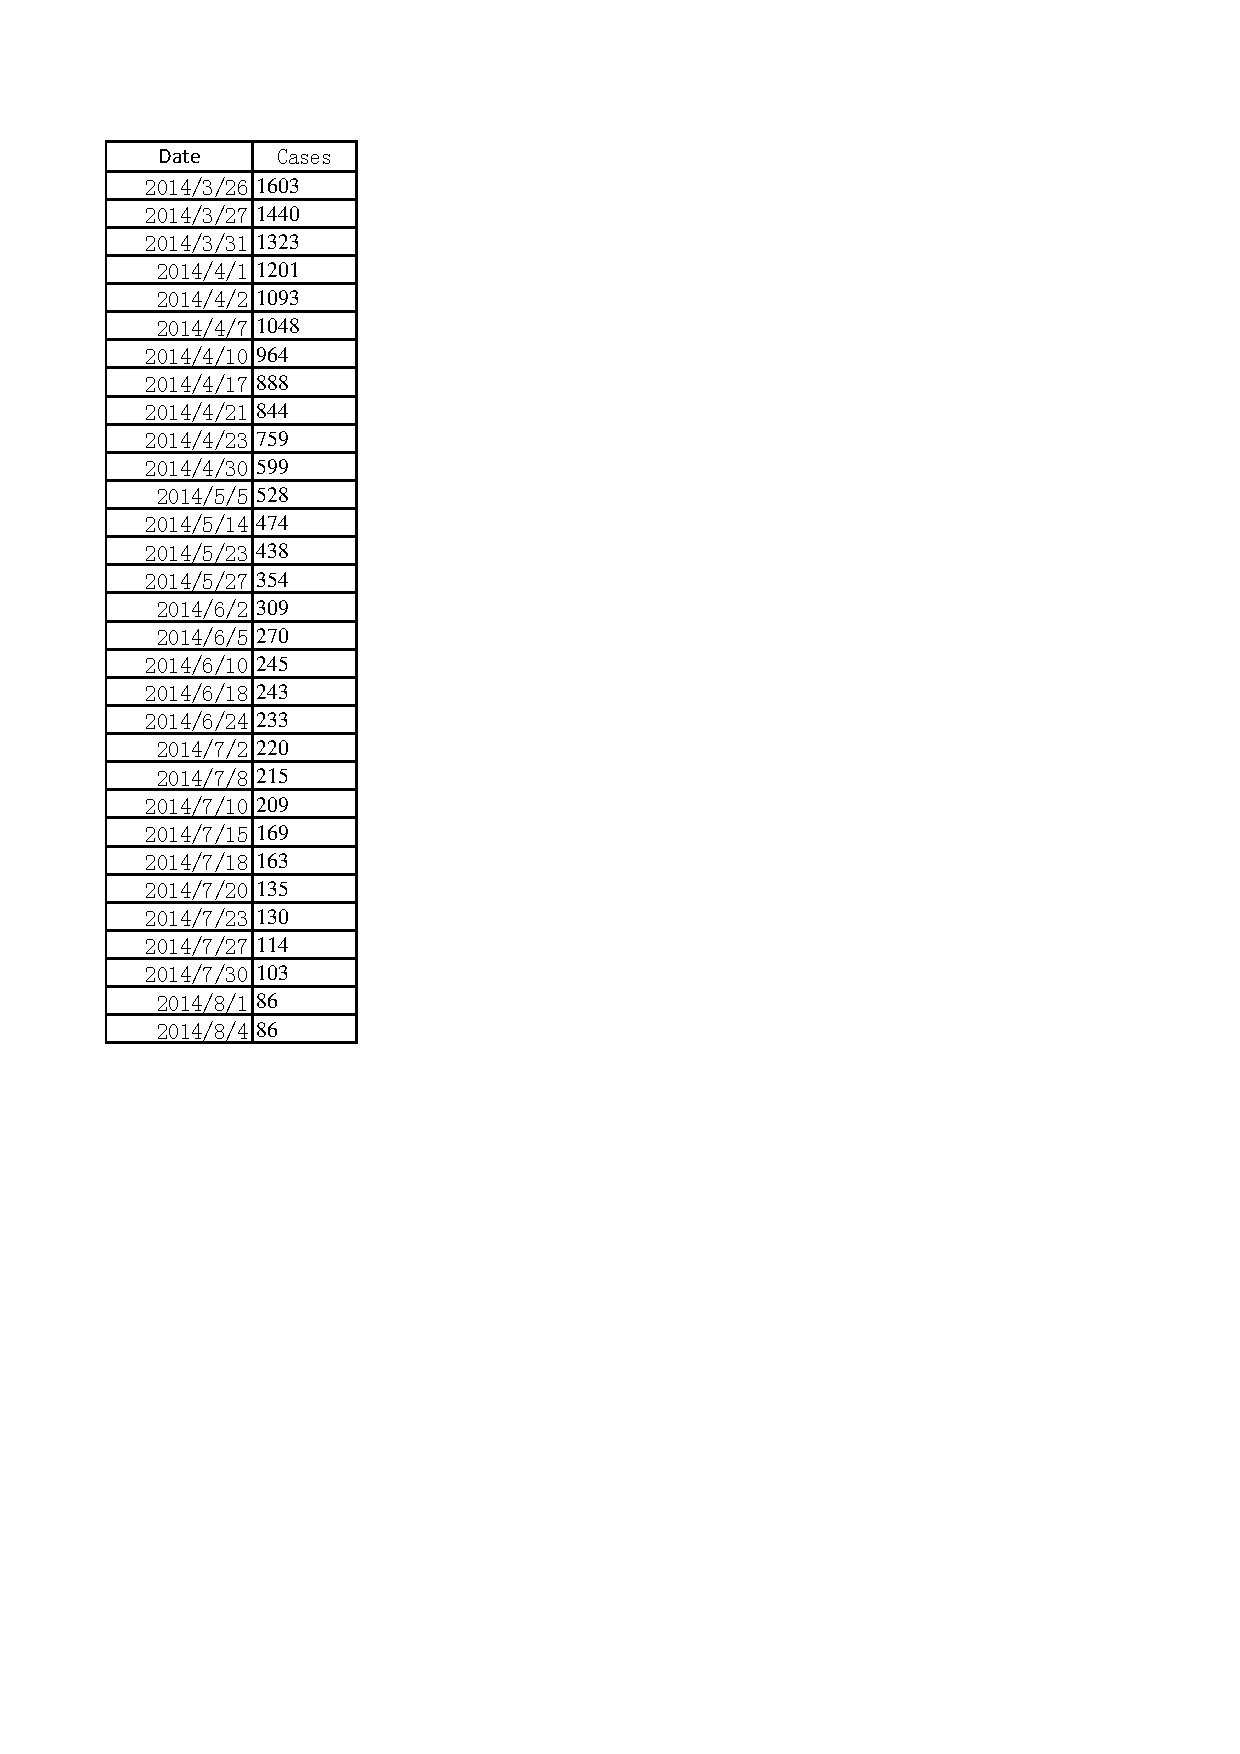
\includegraphics{imgs/statistic.pdf}\nline%
%
